\documentclass[11pt]{article}
\usepackage{amsmath}
\usepackage{amssymb}
\usepackage{geometry}
\usepackage{listings}
\usepackage{enumitem}
\usepackage{graphicx}

\geometry{margin=1in}

% Configuration for SAS code block formatting
\lstset{
    basicstyle=\ttfamily\small,
    breaklines=true,
    xleftmargin=2em
}

\begin{document}

\begin{center}
    {\LARGE \textbf{STAT 505 Assignment Solutions [L1 \& L2]}} \\
\end{center}
\vspace{0.5em}

\begin{enumerate}
    \item The following $n \times p$ data matrix contains $n = 3$ observations for each of $p = 2$ variables $X_1$ (column 1) and $X_2$ (column 2).
    \[
    \begin{bmatrix}
    3 & 18 \\
    8 & 21 \\
    4 & 20
    \end{bmatrix}
    \]
    Calculate each of the following. You can check your work with software, but you should show by hand how the numbers in this case fit into the formula for each.
   

    \begin{enumerate}[label=(\alph*)]
        \item The sample mean vector $\bar{\mathbf{x}}$ \textit{Hint: this is a $2 \times 1$ vector consisting of the sample means for both variables} \\ \\

\begin{figure}[htbp]
    \centering
    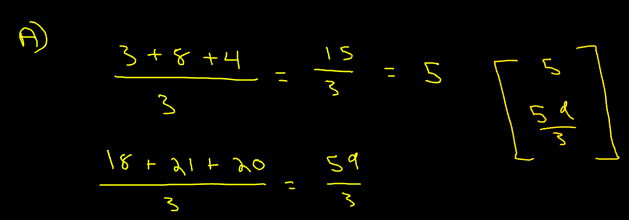
\includegraphics[width=0.6\textwidth]{image6.png} 
    \caption{Handwritten solution for question 1a. }
    \label{fig:handwritten1}
\end{figure}

As shown in Figure \ref{fig:handwritten1}, the sample mean vector is: 

$$ \bar{x}  = \begin{bmatrix} 5 \\ \frac{59}{3} \end{bmatrix} $$

        \item The sample covariance matrix $\mathbf{S}$. Note that we divide by $n - 1$ for this (not $n$). \textit{Hint: this is a $2 \times 2$ matrix consisting of the sample variances for both variables on the diagonals and their covariance on the off-diagonals} \\ \\

\begin{figure}[htbp]
    \centering
    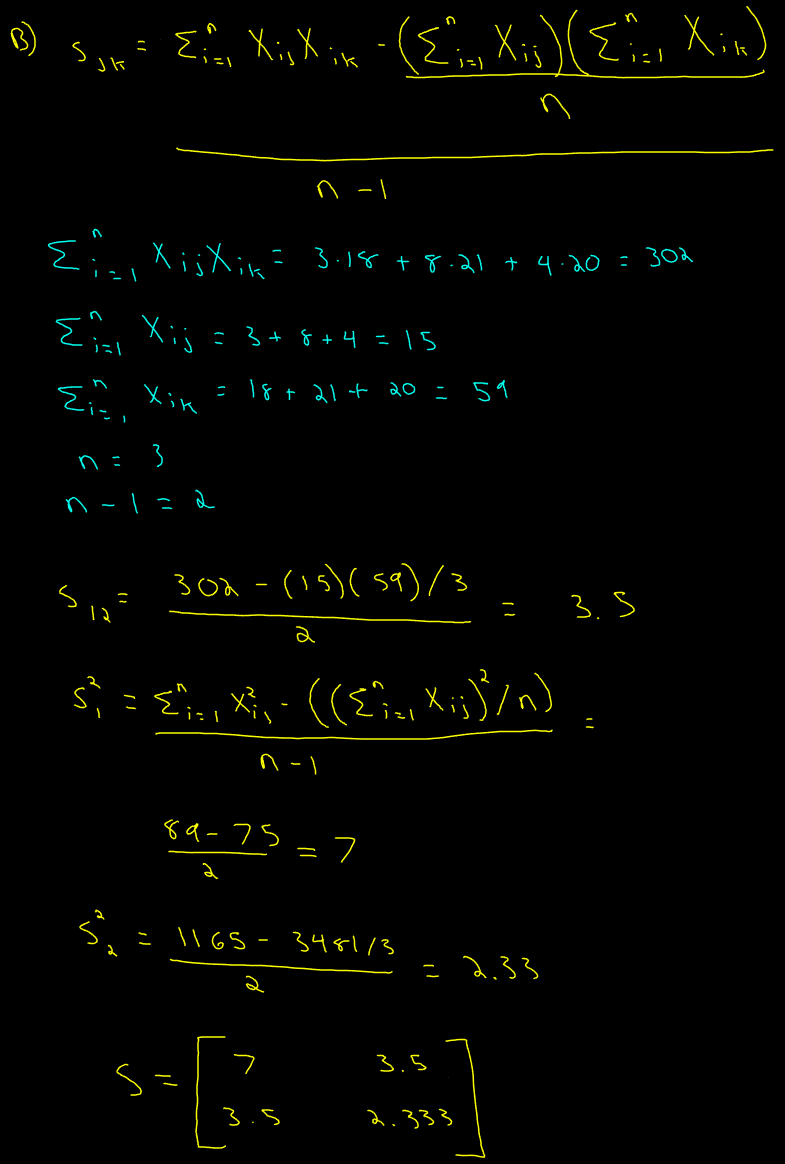
\includegraphics[width=0.6\textwidth]{image7.png} 
    \caption{Handwritten solution for question 1b. }
    \label{fig:handwritten2}
\end{figure}

As shown in Figure \ref{fig:handwritten2}, the sample sample covariance matrix \textbf{S} is:  

$$ S =  \begin{bmatrix}
7 \quad 3.5 \\
3.5\quad 2..333
\end{bmatrix} $$

        \item The sample correlation matrix $\mathbf{R}$  \\ \\


\begin{figure}[htbp]
    \centering
    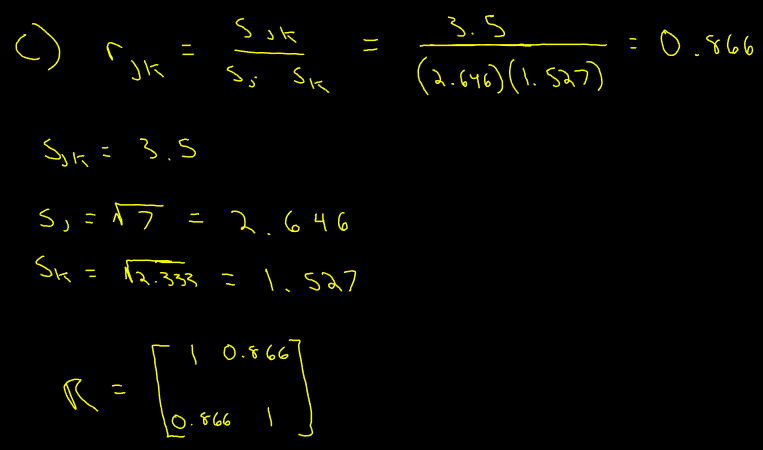
\includegraphics[width=0.6\textwidth]{image5.png} 
    \caption{Handwritten solution for question 1c. }
    \label{fig:handwritten3}
\end{figure}

As shown in Figure \ref{fig:handwritten3}, the sample sample correlation matrix \textbf{R} is:  

$$ R =  \begin{bmatrix}
1 \quad 0.866 \\
0.866 \quad 1
\end{bmatrix} $$

    \end{enumerate}



    \item Let $\mathbf{X}' = [X_1, X_2]$ denote the vector of variables from above, and define $\mathbf{Y}' = [Y_1, Y_2]$ by
    \[
    Y_1 = (X_1 + X_2)/2
    \]
    and
    \[
    Y_2 = X_2 - 2X_1
    \]
    \begin{enumerate}[label=(\alph*)]
        \item Find the coefficient matrix $\mathbf{A}$ such that $\mathbf{Y} = \mathbf{AX}$. \\ \\

\begin{figure}[htbp]
    \centering
    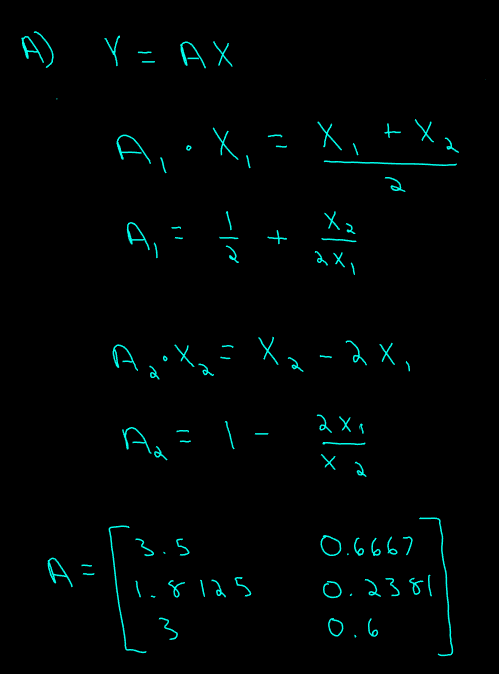
\includegraphics[width=0.6\textwidth]{image4.png} 
    \caption{Handwritten solution for question 2a. }
    \label{fig:handwritten4}
\end{figure}

As shown in Figure \ref{fig:handwritten4}, the coefficient matrix \textbf{A} is:  

$$ A =  \begin{bmatrix}
3.5 \quad 0.6667 \\
1.8125 \quad 0.2381 \\
3 \quad 0.6 \\
\end{bmatrix} $$

        \item Find the sample mean vector and covariance matrix for $\mathbf{Y}$ \\ \\

\begin{figure}[htbp]
    \centering
    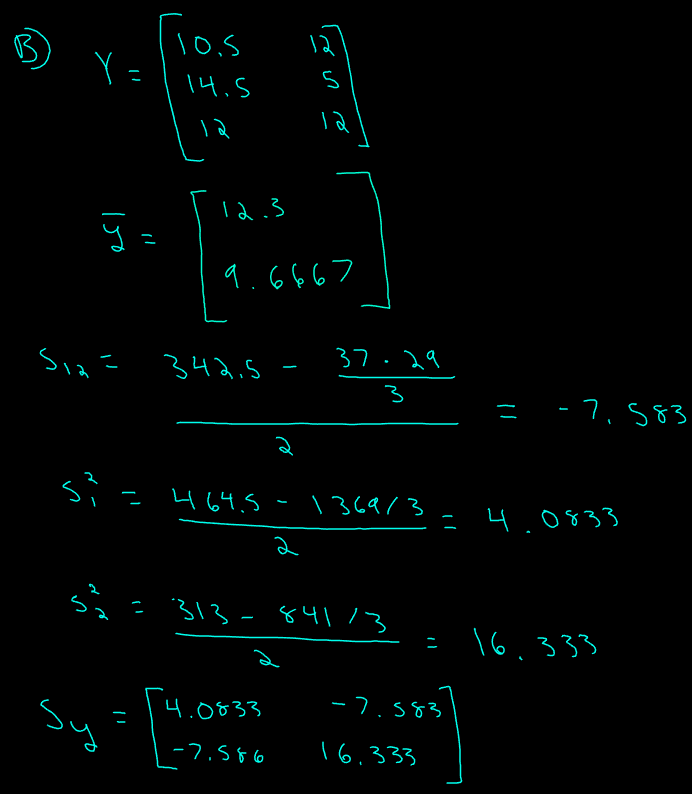
\includegraphics[width=0.6\textwidth]{image3.png} 
    \caption{Handwritten solution for question 2b. }
    \label{fig:handwritten5}
\end{figure}

As shown in Figure \ref{fig:handwritten5}, the sample mean vector and covariance matrix for \textbf{Y} is:  
\footnote{after handwriting, I realized the transposing mistake and corrected in the latex document}
$$ \bar{y} =  \begin{bmatrix}
12.3 \\
9.666
\end{bmatrix} $$
 
$$ S_y=  \begin{bmatrix}
4.0833 \quad -7.583 \\
-7.583 \quad 16.333
\end{bmatrix} $$




    \end{enumerate}

    \item The data ``companies.csv'' is available on our Canvas page and can be read into SAS with the commands below. The variables (columns) are $X_1$, $X_2$, and $X_3$.
    
\begin{lstlisting}
data company;
infile "/companies.csv" delimiter="," firstobs=2;
input x1 x2 x3;
run;
\end{lstlisting}
    \vspace{0.5em}
    Define new variables $Y_1 = X_1 + X_2 + X_3$ and $Y_2 = X_3 - X_1$. Find the mean and variance for each of $Y_1$ and $Y_2$. Also, find the correlation between $Y_1$ and $Y_2$. \\ \\
\end{enumerate}

This is the SAS code used in SAS Online Studio for this question:

\begin{verbatim}
data company;
infile "/home/u64433460/companies.csv" delimiter="," firstobs=2;
input x1 x2 x3;
y1 = x1 + x2 + x3;
y2 = x3 - x1;
run;

proc means data=company mean var;
    var y1 y2;
run;

proc corr data=company plots=none;
    var y1 y2;
run;
\end{verbatim}

The SAS procedures resulted in the following tables that present the mean, variance, and the covariance in figures \ref{fig:SAS1} and \ref{fig:SAS2}.

\begin{figure}[htbp]
    \centering
    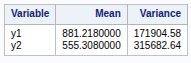
\includegraphics[width=0.3\textwidth]{image2.png} 
    \caption{SAS solution for question 3.1, showing the mean and the variance for $Y_1$ and $Y_2$. }
    \label{fig:SAS1}
\end{figure}

\begin{figure}[htbp]
    \centering
    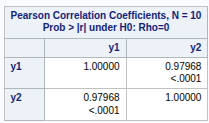
\includegraphics[width=0.3\textwidth]{image1.png} 
    \caption{SAS solution for question 3.2, showing the covariance between $Y_1$ and $Y_2$.}
    \label{fig:SAS2}
\end{figure}

\end{document}
